\documentclass[11pt]{article}

\usepackage[margin=0.89in]{geometry}
\usepackage{titlesec}
\usepackage[hidelinks]{hyperref}
\usepackage{adjustbox}
\usepackage{float}
\usepackage{graphicx} %To include PDF as an image
\usepackage{times}
\usepackage{svg} % To include images in SVG format
\usepackage{ragged2e} % To justify abstract
\usepackage[T1]{fontenc}
\usepackage{comment} % For comment blocks
\usepackage[
    sorting=none
]{biblatex}
\usepackage{amsmath}
\usepackage{longtable}
\addbibresource{references.bib}


\titleformat*{\section}{\large\bfseries}

\begin{document}
\hypersetup{pdfauthor={Prusak, Patryk;}, pdftitle={}}

\title{Prusak_Patryk_ADVML_Project_1}
\author{\normalsize Patryk Prusak }
\hspace{0pt}
\vfill
\begin{center}

    \textbf{\huge{Cyclic Coordinate Descent for Logistic Regression with Lasso regularization}}
    
\end{center}

\vspace{0.5cm}
\begin{center}
    \normalsize{Patryk Prusak}
\end{center}
\vspace{0.5cm}
\begin{center}
    \normalsize{supervisor}\\
    \vspace{0.3cm}
    \normalsize{mgr Katarzyna Woźnica}
\end{center}

\vspace{0.5cm}

\begin{center} 
\normalsize{Warsaw University of Technology} \\
\vspace{0.3cm}
\normalsize{\today} \\
\vspace{0.3cm}
Advanced Machine Learning Course
\end{center}

\vspace{1cm}


\tableofcontents
\vfill
\hspace{0pt}
\newpage

%TODO:
% Every point described below should be included in separate section. Maximal length of report is 6 pages A4 (title page and refernces are not included in the limit). Report should include:
% • Methodology.
% o Selection and generation of datasets.
% o Details about algorithm implementation and applied optimizations
% • Discussion about correctness of the LogRegCCD algorithm.
% Suggested approach to address this point:
% o Performance of the algorithm at lambda=0
% o Likelihood function values and coefficient values depending on iteration
% o Comparison with ready implementation of logistic regression with L1 penalty
% • Impact of dataset parameters: n.p,d,g on the performance of LogRegCCD algorithm.
% • Benchmark of LogRegCCD with LogisticRegression algorithm.
% Suggested approach to address this point:
% o Performance of algorithms regarding different metrics
% o Values of coefficients obtained in these two methods


\section{Selection and generation of datasets}

The implemented Cyclic Coordinate Descent for Logistic Regression with Lasso regularization (LogRegCCD) algorithm was tested on both real and synthetic datasets to evaluate its performance given various metrics such as accuracy, precision, recall, F1 score, balanced accuracy and ROC AUC \cite{powers2011evaluation, brodersen2010balanced, fawcett2006introduction} provided by the scikit-learn \cite{scikit-learn} Python \cite{python} library. \par 



The synthetic datasets have been created with various values of the following parameters: class prior probability $p$, number of samples $n$, number of features $d$, and the covariance matrix $g$ parameter defined as $S[i,j] = g^{|i-j|}$. We have examined all unique combinations of the following parameter values: $p \in \{0.2, 0.3, 0.4, 0.5, 0.6, 0.7, 0.8\}$, $n \in \{1000, 1500, 2000\}$, $d \in \{2, 5, 10, 30\}$ and $g \in \{0.1, 0.3, 0.5, 0.7, 0.9\}$. We have examined more parameter values for $p$ and $g$ to investigate further specific trends discussed in further sections. The synthetic datasets were generated according to the task description, that is:

To generate the dataset, we first draw a binary class variable $Y$ from a Bernoulli distribution with class prior probability $p$. Then, we generate the feature vector $X$ based on the class label. For $Y = 0$, $X$ follows a $d$-dimensional multivariate normal distribution with a mean vector $\boldsymbol{\mu_0} = (0, \dots, 0)$ and a covariance matrix $S$ defined as $S[i,j] = g^{|i-j|}$. For $Y = 1$, $X$ follows a similar multivariate normal distribution but with a mean vector $\boldsymbol{\mu_1} = \left(1, \frac{1}{2}, \frac{1}{3}, \dots, \frac{1}{d} \right)$ while maintaining the same covariance matrix $S$. This process is repeated to generate $n$ observations.


The real datasets were taken from the OpenML \cite{OpenML2013} repository. The datasets were selected based on having the number of features of at least 50\% of the number of samples, preferably numerical features, a low amount of missing values, and a multi-class response variable. The datasets that have met these criteria are as follows:
\begin{itemize}
    \item \textbf{ArrhythmiaDataset} - A binarized version of the Cardiac Arrhythmia Database, aiming to determine the type of arrhythmia from the ECG recordings. This dataset contains 279 features and 452 samples \cite{arrhythmia_5}.
    \item \textbf{SpeechTreatmentDataset} - The dataset contains phonation samples from patients with voice disorders. The dataset assesses whether the voice rehabilitation treatment leads to phonations considered \textit{acceptable} or \textit{unacceptable}. The dataset contains 309 features and 126 samples \cite{lsvt_voice_rehabilitation_282}.
    
    \item \textbf{SemeionDataset} - A binarized version of the Semeion Handwritten Digit Dataset, aiming to determine the digit from the handwritten samples. This dataset contains 256 features and 319 samples (only instances 1 and 0 are considered) \cite{semeion_handwritten_digit_178}.
    \item \textbf{DBWorldSubjectsDataset} - The dataset author collected 64 e-mails from the DBWorld newsletter and used them to train different algorithms to classify between \textit{announces of conferences} and \textit{everything else}. The dataset contains 230 features and 64 samples \cite{dbworld_e-mails_219}.

\end{itemize}

The datasets have been preprocessed by removing colinear features, imputing missing values, and standardizing (min-max scaling for synthetic datasets and unit-variance scaling for real datasets). The datasets were split into training, validation (for the LogRegCCD algorithm), and test sets. The presented results were performed with five predefined seeds, meaning each experiment configuration has been repeated five times.


\section{Details about algorithm implementation and applied optimizations}

Logistic Regression is a machine learning method capable of binary classification. It predicts the probability of an outcome by computing the linear combination of input features and weights and then passing it through the sigmoid function.

The output of the sigmoid function in range $[0,1]$ denotes the probability that the given feature vector $x$ belongs to the positive class. What follows the prediction rule is based on the output of the sigmoid function; if it's larger than a set threshold, such as 0.5, we assign the sample to class 1; otherwise, we assign it to class 0.

To fit the model to the training data, one needs to minimize the loss function, which is, in this case, binary cross-entropy. The model weights must be optimized to find the proper fit; a standard gradient descent algorithm can achieve this.

It is also essential to account for overfitting. Overfitting describes when the trained model can predict samples from the training set very well but struggles on the test set. One method to prevent the model from being overfitted to the training data is Lasso Regularization. In essence, during the training process, the model will also minimize the absolute sum of the coefficients in addition to the loss function. Regularization might result in some of the weights being set to zero, effectively reducing the number of features the model is trained on. Regularization can be helpful when the number of features is vast and some are irrelevant to the prediction task.

To use the Cyclic Coordinate Descent instead of the standard Gradient Descent, one needs to minimize the regularized log-likelihood function using a different algorithm for updating model weights. However, the authors of the 2010 publication entitled \textit{Regularization Paths for Generalized Linear Models via Coordinate Descent} \cite{Friedman2010} present a more sophisticated approach with certain optimizations.


The logistic regression with lasso regularization log-likelihood function is approximated using a quadratic approximation presented in Formula \ref{eq:quadratic-approximation}. The authors also use a regularization path that starts from the largest $\lambda$ where $\beta = 0$ and decreases $\lambda$ gradually, using previous solutions as warm starts. Instead of computing gradients from scratch with each iteration, the authors propose to use covariance updates (Formula \ref{eq:covariance-update}). This, in turn, allows for a more efficient computation of the gradients. For each feature, the optimization problem simplifies to a minimization problem presented in Formula \ref{eq:feature-minimization}.

\begin{equation}\label{eq:quadratic-approximation}
\ell_Q(\beta_0, \beta) = -\frac{1}{2N} \sum_{i=1}^{N} w_i (z_i - \beta_0 - x_i^T \beta)^2 + C
\end{equation}


\begin{equation}\label{eq:covariance-update}
\sum_{i=1}^{N} x_{ij} r_i = \langle x_j, y \rangle - \sum_{k: |\beta_k| > 0} \langle x_j, x_k \rangle \beta_k
\end{equation}

\begin{equation}\label{eq:feature-minimization}
    \min_{\beta_j} \left[ \frac{1}{2} \sum_{i=1}^{N} w_i \left( z_i - \beta_0 - \sum_{k \neq j} x_{ik} \beta_k - x_{ij} \beta_j \right)^2 + \lambda |\beta_j| \right]
\end{equation}

%TODO: this looks ugly, ask if it can stay that way

The algorithm for the cyclic coordinate descent for a given feature $j$ is as follows. Compute partial residuals (excluding $\beta_j$): $r_i = z_i - (\beta_0 + \sum_{k \neq j} x_{ik} \beta_k)$, compute the gradient component $\rho_j$: $\rho_j = \sum_{i=1}^{N} w_i x_{ij} r_i$, apply soft-thresholding for L1 regularization: $\beta_j = \frac{S(\rho_j, \lambda)}{\sum_{i=1}^{N} w_i x_{ij}^2}$, where $S(z, \lambda) = \text{sign}(z) \cdot \max(|z| - \lambda, 0)$ and update $\beta_0$ that is not regularized: $\beta_0 = \frac{\sum_{i=1}^{N} w_i (z_i - x_i^T \beta)}{\sum_{i=1}^{N} w_i}$.


From a high-level overview, the presented algorithm consists of an outer loop where we decrease $\lambda$ along a regularization path, a middle loop where we update the quadratic approximation using the current $(\beta_0, \beta)$, and an inner loop where we perform coordinate descent on the penalized weighted least squares problem. This process has been translated into Python code and is available in the attached notebook.



\section{Impact of dataset parameters: n.p,d,g on the performance of LogRegCCD algorithm}

The performance of the LogRegCCD algorithm was evaluated on synthetic datasets with different values of the parameters: class prior probability $p$, number of samples $n$, number of features $d$, and the covariance matrix $g$ parameter defined as $S[i,j] = g^{|i-j|}$. The results are presented in Figure \ref{fig:synthetic-dataset-parameters}. The performance was evaluated using the following metrics: ROC AUC and balanced accuracy. The general conclusion is that the implemented model performs very similarly to the scikit's LogisticRegression algorithm. Furthermore, the effects of the synthetic dataset features on the performance of the models are as follows:

\begin{itemize}
    \item \textbf{p}: The balanced accuracy decreases as the class prior probability diverges from 0.5. The dataset becomes more imbalanced, and the model struggles to predict the minority class. Meanwhile, for ROC AUC, the effect of the p parameter does not seem to follow a regular pattern. All models achieve the highest ROC AUC for p = 0.5 when the dataset is balanced. For values other than 0.5, ROC AUC drops in a non-regular way.
    \item \textbf{n}: The balanced accuracy increases as the number of samples increases. The model has more data to learn from and can generalize better; for ROC AUC, a similar trend is valid for up to 1500 samples; after that, the ROC AUC stays at a similar level.
    \item \textbf{d}: Both balanced accuracy and ROC AUC increase when the number of features changes from two to five. However, afterward, the performance of the model decreases. This is likely due to the fact that the model is overfitting to the training data. The model has too many features to learn from and starts memorizing the training data instead of generalizing it. This is especially evident in ROC AUC of the logistic regression without regularization.
    \item \textbf{g}: Here, we see a tilted U-shaped curve; as the covariance increases, the balanced accuracy decreases until around 0.7, where balanced accuracy rises rapidly. When the covariance between the features is low, they contribute relatively independently to the classification. As the covariance increases, the features become more correlated, leading to redundant information, and the model's performance worsens. However, around $g \approx 0.7$, a transition happens where the features become so correlated that they effectively act as a smaller number of independent features. At this point, the model starts performing better again. The ROC AUC metric behaves similarly.
    
\end{itemize}

\begin{figure}[h]
    \centering
  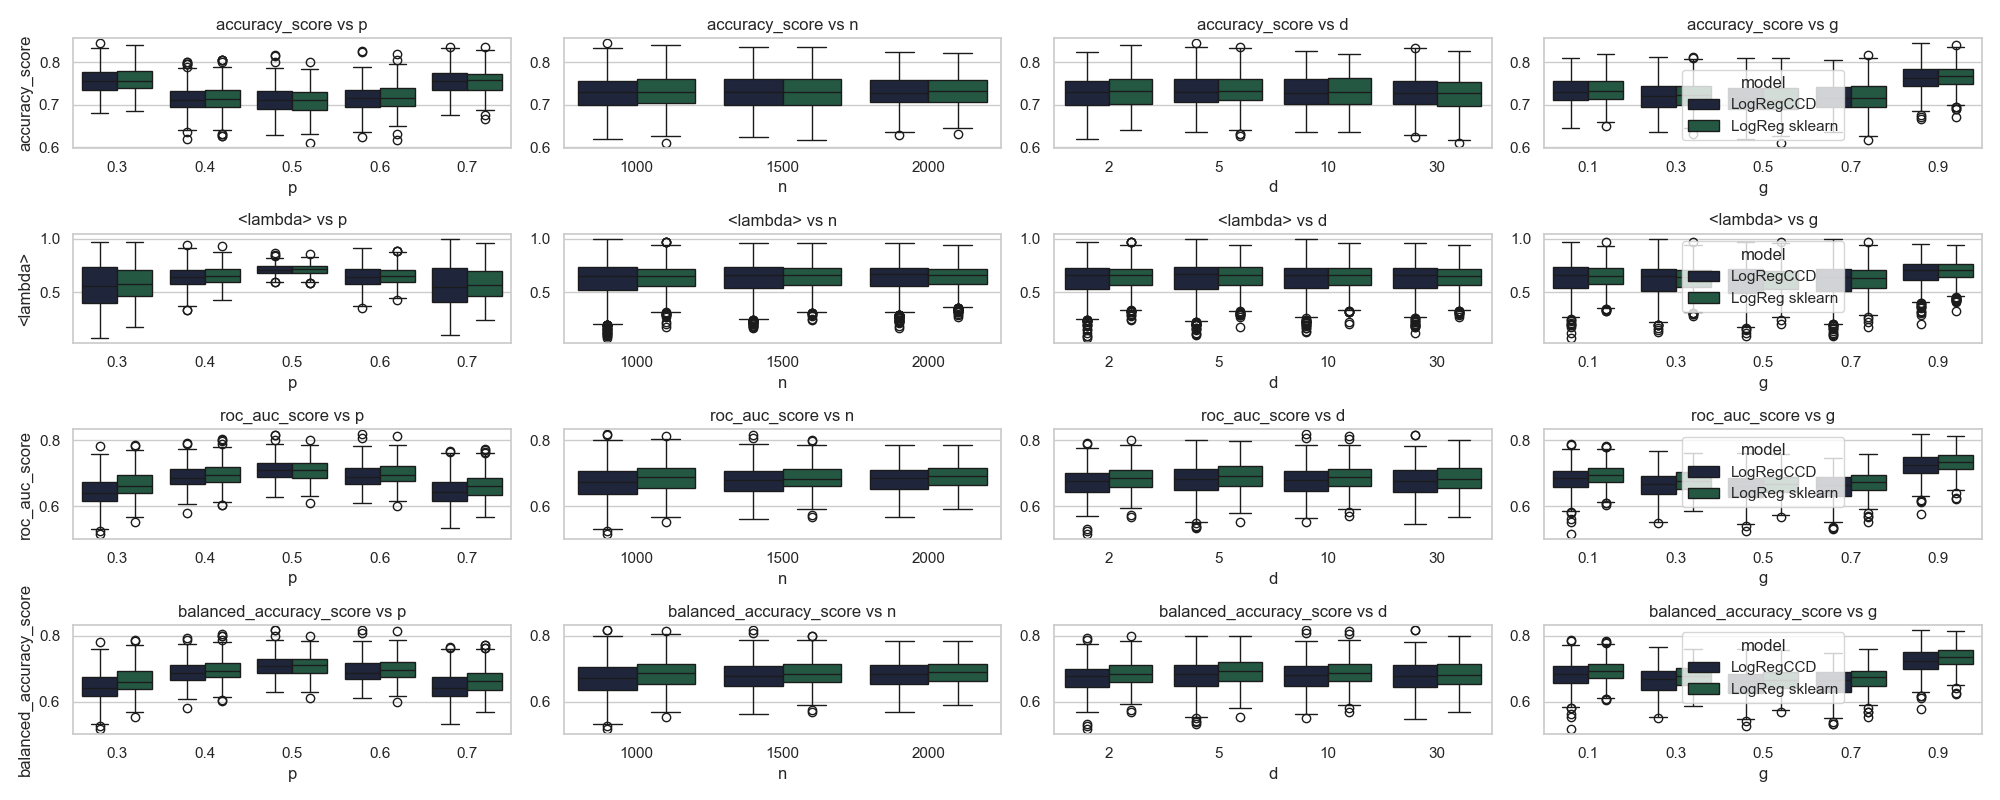
\includegraphics[width=\textwidth]{../results/parameter_facet_grid.png}
    \caption{impact of synthetic dataset parameters on the performance of LogRegCCD algorithm}
    \label{fig:synthetic-dataset-parameters}
  \end{figure}

\section{Benchmark of LogRegCCD with LogisticRegression algorithm}

The overall performance comparison of all three models on the real datasets is available in Figure \ref{fig:real-data-boxplots}. The LogRegCCD algorithm performs nearly identically to the scikit's logistic regression with the l1 penalty. However, in the case of ArrhythmiaDataset and SpeechTreatmentDataset, it achieves higher results in terms of ROC AUC, balanced accuracy, and recall while having slightly worse precision, meaning that the LogRegCCD is better at predicting the positive class in these specific cases. Interestingly, standard logistic regression without penalty performs best regarding all metrics on the DBWorldSubjectsDataset dataset. However, it is essential to remember that this dataset is tiny, and the model might be overfitting the training data. Regardless, here, the LogRegCCD also achieves satisfactory results with accuracy in the neighborhood of 80\%. In some cases, such as the SemeionDataset, the models are able to achieve perfect precision and recall, again this is most likely due to the small size of the dataset. Because of how the algorithm works (separately performs calculations for each feature), we have tried to choose datasets of smaller size. Otherwise, the algorithm would take too long to compute.\par

Similar conclusions can be drawn from the overall comparison of synthetic datasets depicted in Figure \ref{fig:comparison-synthetic-dataset}. The LogRegCCD algorithm performs similarly to the scikit's logistic regression with l1 penalty and without penalty. A notable difference is that in terms of accuracy, Scikit's model with the l1 penalty performs somewhat better than the LogRegCCD algorithm. In contrast, the LogRegCCD algorithm performs marginally better in precision and Scikit's model without penalty, achieving slightly higher balanced accuracy on average. As a result, one might conclude that depending on the metric of interest, it is worthwhile to consider a different model; however, the differences are negligible, and it is more important to choose the model best suited for the specific dataset and task at hand. \par


\begin{figure}[h]
    \centering
  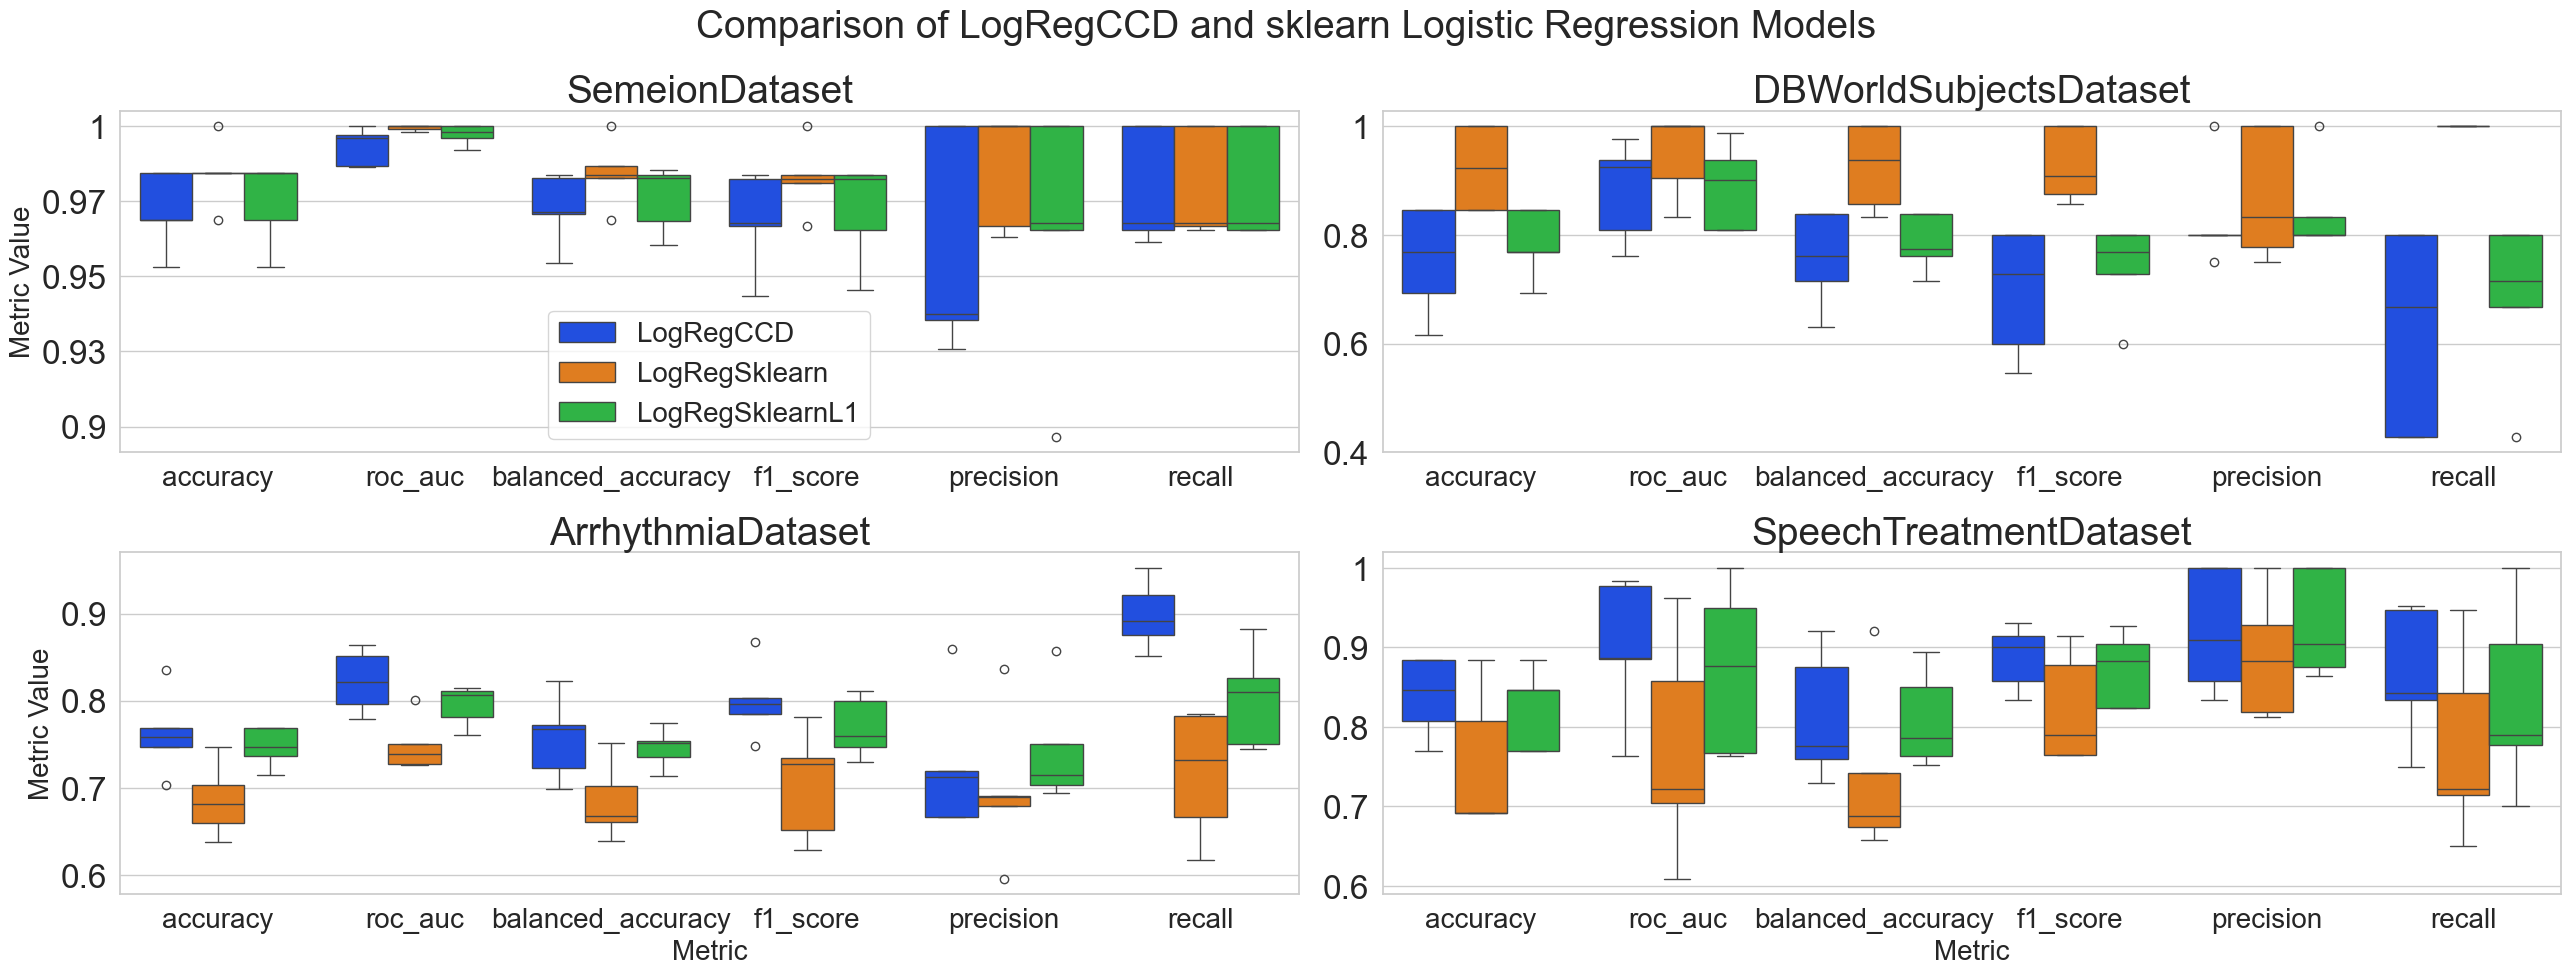
\includegraphics[width=\textwidth]{../results/real_data_boxplots.png}
    \caption{Boxplots of metrics for real datasets}
    \label{fig:real-data-boxplots}
  \end{figure}

\begin{figure}[h]
    \centering
  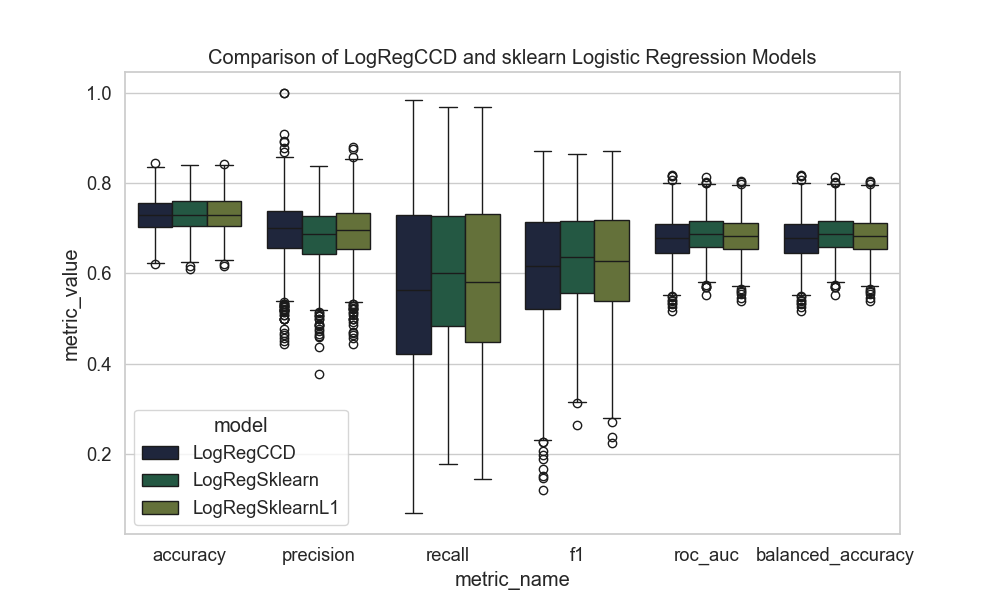
\includegraphics[width=\textwidth]{../results/comparison-synthetic-dataset.png}
    \caption{Comparison of LogRegCCD and LogisticRegression on synthetic dataset}
    \label{fig:comparison-synthetic-dataset}
  \end{figure}

% \subsection{Values of coefficients obtained in these two methods}
%TODO: What should be here? Isn't it already contained in the comparison to L1?


\section{Discussion about the correctness of the LogRegCCD algorithm}

The previous results already hint at the correctness of the implemented algorithm in terms of its similar performance to Scikit's logistic regression. However, to investigate the correctness of the algorithm further, we can look at the log-likelihood function values and coefficient values, depending on iteration. The log-likelihood function measures how well the model fits the data. The higher the value, the better the fit. The coefficient values are the weights assigned to each feature in the model. The higher the value, the more important the feature is for the prediction task. \par

At lambda = 0, the log-likelihood function values and coefficient values depending on iteration are presented in Figure \ref{fig:log-likelihood-synthetic-dataset-lambda-0} and Figure \ref{fig:coefficients-synthetic-dataset-lambda-0} respectively. The log-likelihood function values increase with each iteration, meaning the model improves with each step. Similarly, the coefficient values change with each iteration but stabilize after around 100 iterations. Although the iteration limit is set to 1000, the process stops at around 250 iterations, meaning the model successfully converges. This is a good indicator that the implemented model is correct.\par


\begin{figure}[h]
    \centering
    \begin{minipage}{0.48\textwidth}
        \centering
        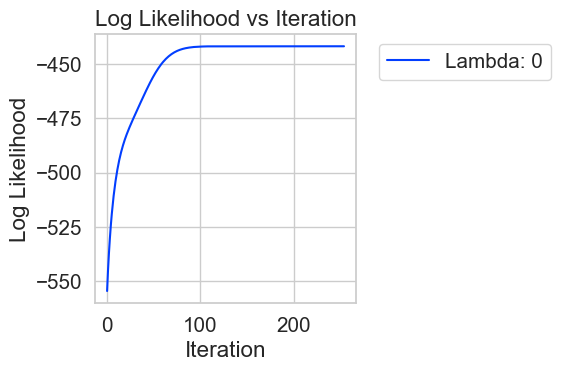
\includegraphics[width=\textwidth]{../results/log_likelihood_synthetic_dataset_lambda_0.png}
        \caption{Log likelihood function values depending on iteration for a synthetic dataset with $\lambda=0$}
        \label{fig:log-likelihood-synthetic-dataset-lambda-0}
    \end{minipage}
    \hfill
    \begin{minipage}{0.48\textwidth}
        \centering
        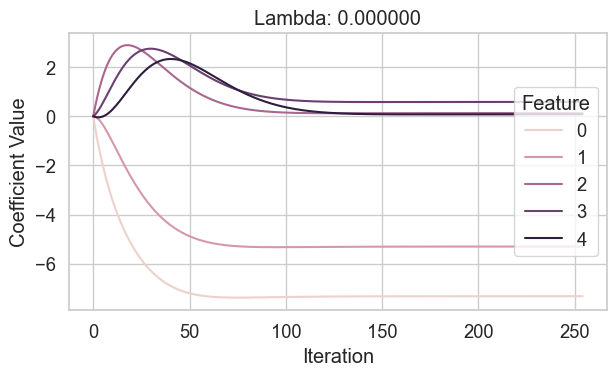
\includegraphics[width=\textwidth]{../results/coefficients_synthetic_dataset_lambda_0.png}
        \caption{Coefficient values depending on iteration for a synthetic dataset with $\lambda=0$}
        \label{fig:coefficients-synthetic-dataset-lambda-0}
    \end{minipage}
\end{figure}

It is worth examining the likelihood function values depending on the iteration per every lambda. This is depicted in Figure \ref{fig:log-likelihood-synthetic-dataset}. The log-likelihood function values increase with each iteration for each lambda. However, the most substantial changes happen for the largest initial lambda value (given that the regularization parameter is not too strong). As the lambda decreases, the log-likelihood function values increase more slowly. This can be explained by the fact that larger lambda causes more aggressive weight changes, translating to significant jumps in log-likelihood. As the lambda values get smaller, the weights are less constrained, and the log-likelihood function values increase more slowly. The same pattern can be observed regarding the coefficient values (Figure in the attached Python notebook). \par 


\begin{figure}
    \centering
  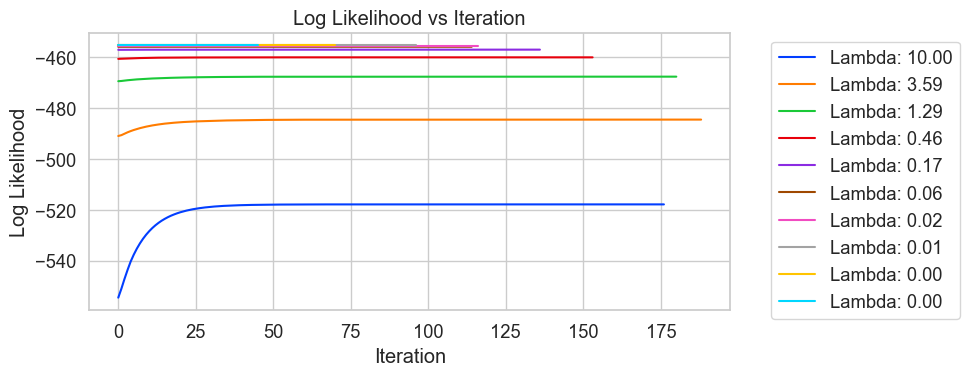
\includegraphics[width=\textwidth]{../results/log_likelihood_synthetic_dataset.png}
    \caption{Log likelihood function values depending on iteration for synthetic dataset}
    \label{fig:log-likelihood-synthetic-dataset}
\end{figure}


Lastly, to investigate the effects of regularization, the values of coefficients based on lambda have been compared with those obtained from the scikit's logistic regression with the l1 penalty. Both models have been tested on a specially prepared dataset with five informative features and five redundant features. The results are presented in Figure \ref{fig:comparison-synthetic-dataset-redundant-features}. To start, both models correctly identify informative features reflected in these features having large coefficient values, whereas the redundant features are close to 0. The two plots are almost identical, with slight differences in what lambda value the coefficients change from zero. This is likely because the scikit's logistic regression uses a different algorithm to compute the coefficients. However, the differences are minor, further strengthening the argument that the implemented algorithm is correct. \par


\begin{figure}[h]
    \centering
  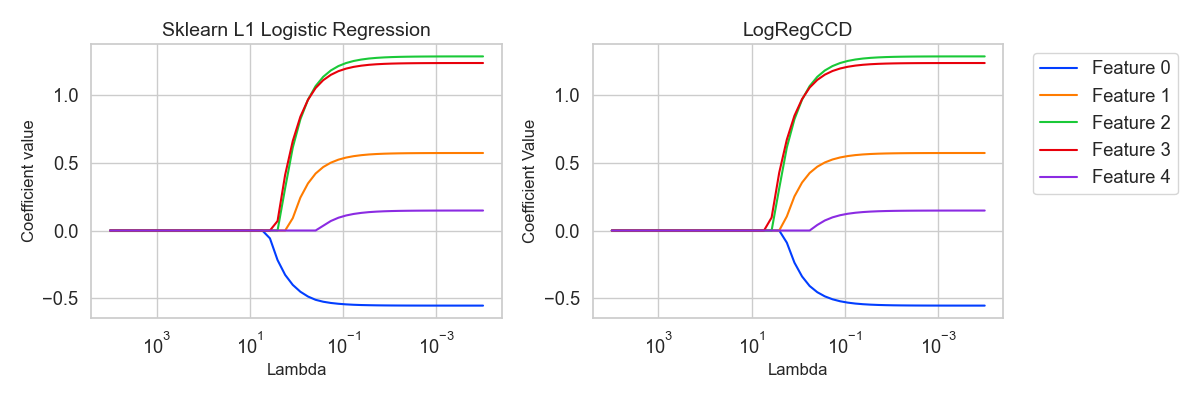
\includegraphics[width=\textwidth]{../results/logistic_regression_l1_logregccd_coefficients_redundant_features.png}
    \caption{Comparison of LogRegCCD and LogisticRegression on a synthetic dataset with redundant features}
    \label{fig:comparison-synthetic-dataset-redundant-features}
  \end{figure}


To conclude, it is fair to say that the implemented algorithm is correct in the given context, meaning that it can perform logistic regression with lasso regularization and performs similarly to the scikit's implementation. The algorithm can converge to a solution, and the results are consistent with the expected behavior of the model. Further information, such as the behavior of the differences in coefficients between the models or the exact coefficient values in different scenarios, is available in the attached Python notebook.


\clearpage 
\listoffigures
% \listoftables
\printbibliography

\end{document}
